\section{Постановка задачи}

\begin{frame}[t]{Исследование пещер}


    \begin{columns}[T,onlytextwidth]
        \begin{column}{0.59\textwidth}
            \small
                \textbf{Цель} --- добыча природных минералов, поиск исторических и археологических находок.
            \begin{exampleblock}{Непроходимые места для человека}
                \begin{itemize}
                    \item Узкие галереи, огромные пропасти, обвалы, сифоны
                    \item Скопление угарного газа
                    \item Потеря ориентации в пространстве
                \end{itemize}
            \end{exampleblock}
            \vspace{-0.2cm}
            \begin{alertblock}{Заинтересованные стороны}
                \begin{enumerate}
                    \item Военные --- \textit{Darpa Subterranean Challenge}
                    \item Ученые --- "Горный институт Уральского отделения РАН", 
                    \item Космические агентства --- ESTEC (DAEDALUS), Роскосмос (FEDOR), NASA (CADRE)
                \end{enumerate}
            \end{alertblock}
        \end{column}
        \begin{column}{0.39\textwidth}
            \begin{figure}[H]
                \begin{subfigure}{0.49\textwidth}
                    \centering\includegraphics[height=2cm,width=1\textwidth,keepaspectratio]{../images/slides/rip.jpg}
                    \caption{Могила в пещере}
                \end{subfigure}
                \begin{subfigure}{0.49\textwidth}
                    \centering\includegraphics[height=2cm,width=1\textwidth,keepaspectratio]{../images/surface_types/siphon.png}
                    \caption{Сифоны}
                \end{subfigure}
            
                \begin{subfigure}{0.49\textwidth}
                    \centering\includegraphics[height=2cm,width=1\textwidth,keepaspectratio]{../images/slides/daedalus.jpg}
                    \caption{DAEDALUS для исследования пещер на луне}
                \end{subfigure}
                \begin{subfigure}{0.49\textwidth}
                    \centering\includegraphics[height=2cm,width=1\textwidth,keepaspectratio]{../images/open_cave.jpg}
                    \caption{DARPA Subterranean Challenge}
                \end{subfigure}
            \end{figure}
        \end{column}
    \end{columns}
\end{frame}

\note{Текст}

\begin{frame}[t]{Предментая область: Пещеры}
    \framesubtitle{}
    \vspace{-0.8cm}
    \begin{figure}[H]
        \begin{subfigure}{0.49\textwidth}
            \begin{subfigure}[b]{0.49\textwidth}
                \centering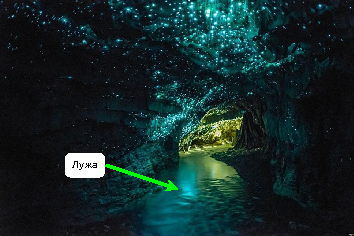
\includegraphics[height=2.5cm,width=1\textwidth,keepaspectratio,page=1]{./tikz_pictures.pdf}
                \caption{Лужа}
            \end{subfigure}
            \hfill
            \begin{subfigure}[b]{0.49\textwidth}
                \centering\includegraphics[height=2.5cm,width=1\textwidth,keepaspectratio]{surface_types/moss.jpg}\\
                \caption{Мох}
            \end{subfigure}

            \begin{subfigure}[b]{0.49\textwidth}
                \centering\includegraphics[height=2.5cm,width=1\textwidth,keepaspectratio]{surface_types/salt.jpg}\\
                \caption{Твердые породы}
            \end{subfigure}
            \begin{subfigure}[b]{0.49\textwidth}
                \centering\includegraphics[height=2.5cm,width=1\textwidth,keepaspectratio]{surface_types/sand.jpg}\\
                \caption{Земля}
            \end{subfigure}
            \caption*{Типы опорных поверхностей}
        \end{subfigure}
        \begin{subfigure}{0.49\textwidth}
            \begin{subfigure}{0.99\textwidth}
                \centering\includegraphics[height=3cm,width=1\textwidth,keepaspectratio]{../images/human_crawling.png}
                \caption*{Габариты пещеры (Свободная узость)}
            \end{subfigure}

            \begin{subfigure}{0.99\textwidth}
                \centering\includegraphics[height=3cm,width=1\textwidth,keepaspectratio]{../images/cave_maps/map3.png}
                \caption*{Протяженность пещер: 1--2 км}
            \end{subfigure}
        \end{subfigure}
    \end{figure}
\end{frame}

\note{Предметной областью являются пещеры. Слева представлены типы опорных поверхностей, которые могут встречаться в пещерах и были рассмотрены в данной работе. Это земляной грунт, малые водяные препятствия или лужи, твердые породы, а также мох.

Для разработки объекта исследования необходимо понимать также и габариты пещер, а также их протяженность. Изучив различные карты пещер, такие как на рисунке внизу - было решено взять протяженность пещер в диапазоне от 1 до 2ух км.

Так как наша основная задача это исследовать пещеры, которые не может исследовать человек физически из-за ограничения размеров. Человеку сложно долго ползать на четвереньках, поэтому я решил так, что робот должен быть как минимум меньше, чем средний мужчина в габаритах. А именно 600х1000х600 мм.

Теперь мы можем сделать первичную постановку задачи для методов.
}

\begin{frame}[t]{Вопрос: Как картографировать поверхность под лужей?}
    \framesubtitle{}
    \vspace{-1cm}
    \begin{columns}[T,onlytextwidth]
        \begin{column}{0.44\textwidth}
        \end{column}
        \begin{column}{0.44\textwidth}
            \begin{figure}[H]
                \begin{subfigure}[b]{0.9\textwidth}
                    \centering
                    \centering\includegraphics[height=3.5cm,width=1\textwidth,keepaspectratio,page=2]{./tikz_pictures.pdf}
                \end{subfigure}

                \begin{subfigure}{0.8\textwidth}
                    \centering\includegraphics[height=2cm,width=1\textwidth,keepaspectratio]{terrain_w_water_camera.png}
                    \caption*{Вид с камеры}
                \end{subfigure}
            \end{figure}
        \end{column}
    \end{columns}
\end{frame}

\note{Несколько слов о преимуществе построения карты с помощью ощупывания, относительно оптических методов. Пример на слайде. Задача - построить карту поверхности, она на левой картинке. Но над поверхностью находится вода. Так вот, лидар будет отражаться от поверхности и построит гладую поверхность, а камера не будет работать в мутной воде, как и зеленый лидар.

С использованием же разработанных методов, данная задача решаема, что и будет показано далее.
}

\begin{frame}[t]{Цель работы}
    \framesubtitle{}
    Разработать \textbf{метод построения карты местности} с определением \underline{геометрических} и \underline{физико-механических} свойств \textit{опорной поверхности} роботом с шагающими движителями снабженными \underline{тактильными датчиками}, \textit{без использования оптических сенсоров}.
    \begin{figure}[H]
        \begin{subfigure}{0.49\textwidth}
            \centering\includegraphics[height=3.5cm,width=1\textwidth,keepaspectratio]{conv_concave.png}
            \caption*{Определение геометрических свойств}
        \end{subfigure}
        \begin{subfigure}{0.49\textwidth}
            \centering\includegraphics[height=3.5cm,width=1\textwidth,keepaspectratio]{s_shape_leg/view.jpg}
            \caption*{Определение физических свойств}
        \end{subfigure}
    \end{figure}
\end{frame}

\note{Целью работы являлось разработать метод построения карты местности роботом с шагающими движителями, у которого на стопах установлены датчики силы. Задача должна решаться без использования оптических сенсоров.

Я разбил понятие построения карты на две задачи: определение геометрических свойств и физико - механических.

Прежде чем говорить более конкретно об этих задачах, нужно вначале определить предметную область, так как она сильно влияет на постановку задачи.}

\begin{frame}[t]{"1, 2" Построение рельефа местности}
    \framesubtitle{}
    \begin{columns}[T,onlytextwidth]
        \begin{column}{0.49\textwidth}
            \textbf{Геометрические свойства:}\\
            \textit{Входные данные}: следовая дорожка, представленная в виде облака точек.

            \textit{Выходные данные}: полигональная сетка и плотное облако точек.

            \textit{Допустимая точность}: 0.1 м
            \begin{figure}[H]
                \begin{subfigure}[t]{0.49\textwidth}
                    \centering\includegraphics[height=2cm,width=1\textwidth,keepaspectratio]{../images/slides/surface_research.png}
                    \caption{Исследуемая поверхность}
                \end{subfigure}
                \begin{subfigure}[t]{0.49\textwidth}
                    \centering\includegraphics[height=2cm,width=1\textwidth,keepaspectratio]{../images/slides/result_research.png}
                    \caption{Следовая дорожка и полигональная сетка}
                \end{subfigure}
            \end{figure}
        \end{column}
        \begin{column}{0.49\textwidth}
            \textbf{Физико-механические свойства:}\\
            \textit{Входные данные}: обученный классификатор поверхностей, данные с внутренних датчиков робота.

            \textit{Выходные данные}: процентное соотношение упругих, твердых и пластичных свойств пройденной поверхности.

            \textit{Допустимая ошибка}: 20\% 

            \vspace{-0.35cm}
            \begin{figure}[H]
                \begin{subfigure}{0.49\textwidth}
                    \centering\includegraphics[height=2cm,width=1\textwidth,keepaspectratio]{../images/slides/avg_lin_vel_rev_min.png}
                    \caption*{Пример данных для обучения}
                \end{subfigure}
                \begin{subfigure}{0.49\textwidth}
                    \centering\includegraphics[height=2cm,width=1\textwidth,keepaspectratio]{../images/slides/data.png}
                    \caption*{Пример поверхности}
                \end{subfigure}
            \end{figure}
        \end{column}
    \end{columns}
\end{frame}

\note{\scriptsize Рассматривая геометрические свойства, то входными данными я считаю следовую дорожку, которая представлена в виде облака точек, относительно абсолютных систем координат.

Результатом примененного метода решения должны получиться полигональная сетка пройденной поверхности, а также плотное облако точек. Эти представления являются типичными способами представления для работы с навигацией.

Допустимой точностью является 5 сотых метра. Такая точность была взята из протяженности пещеры и осознанием того, что данный метод может предложить только первичное представление о поверхности и не может конкурировать с оптическими способами построения карты. На рисунке представлены примеры входных и выходных данных. Синим цветом отмечена следовая дорожка.

Целью же определения физико-механических свойств является получение процентного соотношения упругих, твердых и пластичных свойств пройденной поверхности, когда на вход метод получает данные только с проприоцептивных сенсоров. Для решения этой задачи необходимо обучить модель машинного обучения. На рисунках представлен одна из зависимостей, которую можно использовать для обучения, а также пример исследуемой поверхности. К примеру при одинаковой угловой скорости, робот движется с разной линейной скоростью, в зависимости от материала.

Ошибка в 20 процентов была взята из-за частого обновления результатов, так как робот будет заново выдавать результат каждые 200 шагов.

Более точные формулировки задач с идеей решения и принятыми предположениями будут далее.}

\begin{frame}[t]{Объект исследования}
    \framesubtitle{}
    \begin{columns}[T,onlytextwidth]
        \begin{column}{0.54\textwidth}
            \textbf{Класс многоногих шагающих роботов} с 
            а) Цельным или сочленённым корпусом
            б) Цикловыми движителями с одной степенью свободы, управляемые зависимо или независимо друг от друга.

            \textit{Требования к данному классу}:
            \begin{itemize}
                \item Компактные размеры (меньше чем $1000\times600\times600$ мм)
                \item Залезать на препятствия высотой меньше, чем $\frac{3}{4}$ длины корпуса
                \item Преодолевать представленные
                      опорные поверхности
            \end{itemize}
        \end{column}
        \begin{column}{0.44\textwidth}
            \begin{figure}[H]
                \hfill
                \begin{subfigure}{0.99\textwidth}
                    \centering\includegraphics[height=2cm,width=1\textwidth,keepaspectratio]{from_master/whegs2.jpg}
                    \caption{WHegs}
                \end{subfigure}

                \hfill
                \begin{subfigure}{0.49\textwidth}
                    \centering\includegraphics[height=2cm,width=1\textwidth,keepaspectratio]{from_master/rhex.jpg}
                    \caption{Boston Dynamics RHex}
                \end{subfigure}
                \begin{subfigure}{0.49\textwidth}
                    \centering\includegraphics[height=2cm,width=1\textwidth,keepaspectratio]{from_master/gakken.jpg}
                    \caption{Gakken Centipede}
                \end{subfigure}
            \end{figure}
        \end{column}
    \end{columns}
\end{frame}

\note{Рассмотрев различные варианты роботов, было решено выбрать класс многоногих шагающих роботов с цельным или сочлененным корпусом и цикловыми движителями с одной степенью свободы, управляемые зависимо или независимо друг от друга.

Такой класс был выбран так как его представители показывают высокие показания профильной проходимости, что видно в видео справа. На рисунках представлены разные представители - вхегс, рхекс, сентипеде.

Нужно, чтобы разработанный роботом меньше габаритов пещеры, мог залезать на препятствия высотой меньше, чем ¾ длины корпуса, а также мог физически преодолевать препятствия, которые были заявлены как те, которые можно встретить в пещере.
}

\begin{frame}[t]{"3" Оптимизация кинематической схемы}
    \framesubtitle{}
    \begin{columns}[T,onlytextwidth]
        \begin{column}{0.49\textwidth}
            Решить $F=f(x) \rightarrow max$ критерий оптимизации, где

            $f(x)$ --- критерии: пройденная дистанция, длина корпуса\\
            $(x)$ --- параметр: количество ног

            \textit{Количество ног имеет прямую зависимость с длиной корпуса робота.}
        \end{column}
        \begin{column}{0.49\textwidth}
            \vspace{-0.5cm}
            \begin{figure}[H]
                \begin{subfigure}{0.99\textwidth}
                    \centering\includegraphics[height=1.8cm,width=1\textwidth,keepaspectratio]{f1.png}
                    \caption*{Кол-во ног $\uparrow$, детализация поверхности $\uparrow$}
                \end{subfigure}

                \begin{subfigure}{0.99\textwidth}
                    \centering\includegraphics[height=1.8cm,width=1\textwidth,keepaspectratio]{f2.png}
                    \caption*{Длина робота $\uparrow$, курсовая проходимость $\downarrow$}
                \end{subfigure}

                \begin{subfigure}{0.99\textwidth}
                    \centering\includegraphics[height=1.8cm,width=1\textwidth,keepaspectratio]{f3_new.png}
                    \caption*{Длина робота $\uparrow$, проходимость $\uparrow$}
                \end{subfigure}
            \end{figure}
        \end{column}
    \end{columns}
\end{frame}

\note{Как можно было заметить, у различных представителей этого класса, разное количество ног. Более того, количество ног также влияет и на построение карты, так как если у робота ног больше, то карта будет более детализированной, а следовательно - точнее. Но с другой стороны пещеры имеют много изгибов и при большой длине он может застрять. Более длинный робот может преодолевать больше препятствий, как это показано на рисунке. Нужно сделать ремарку, что количество ног напрямую влияет на длину робота в данном классе движителя.

Следовательно у нас возникает мульти критериальная задача оптимизации, где критерием является пройденная дистанция и длина корпуса. И задача - определить оптимальное количество ног.
}

\begin{frame}[t]{"4" Верификация преобразователя силы}
    \framesubtitle{}
    \begin{columns}[T,onlytextwidth]
        \begin{column}{0.49\textwidth}
            Охарактеризовать материал для случаев, когда площадь приложения силы меньше, чем площадь активной части сенсора.

            \textit{Входные данные}: показания разработанного датчика и значение реально приложенной нагрузки

            \textit{Выходные данные}: разница между нормализованным значением с датчика и реальной нагрузкой

            \textit{Допустимая ошибка}: 10\% 
        \end{column}
        \begin{column}{0.49\textwidth}
            \begin{figure}[H]
                \begin{subfigure}{0.9\textwidth}
                    \centering\includegraphics[height=2cm,width=1\textwidth,keepaspectratio]{velostat_sensor.jpg}
                    \caption{Материал Velostat}
                \end{subfigure}

                \begin{subfigure}{0.9\textwidth}
                    \centering\includegraphics[height=2cm,width=1\textwidth,keepaspectratio]{simplest_sensor.jpg}
                    \caption{Простейший преобразователь силы}
                \end{subfigure}
            \end{figure}
        \end{column}
    \end{columns}
\end{frame}

\note{В первичной постановке задачи о построении карты, как для определения геометрических, так и физико-механических свойств, говорилось о том, что на роботе установлены датчики силы. После обзора различных решений, было решено разработать свой пьезорезистивный преобразователь силы на основе Velostat. Данный материал был выбран из-за его отличного соотношения цена/качество. Так как на робота нужно установить много датчиков на каждую ногу, это является важным фактором.

При изучения данного материала я заметил, что когда площадь приложения силы меньше, чем площадь активной части сенсора, то при одинаковом давлении, показания будут разными. А это будет сильно влиять на работу алгоритмов. Примером является маленький камушек, на который робот наехал при ходьбе.

Поэтому было решено охарактеризовать преобразователь для данной задачи. Допустимая ошибка в 10 процентов взята из принятой ошибки в физических экспериментах.
}

\begin{frame}[t]{Структура}
    \framesubtitle{}
    \begin{figure}[H]
        \centering\includegraphics[height=6.5cm,width=1\textwidth,keepaspectratio]{main_diag_hor.png}
    \end{figure}
\end{frame}

\note{Но вначале нужно ограничить мое место в разработке данной робототехнической системы. На экране структура проекта, где оранжевым цветом представлено то, что было разработано мной и где есть научная новизна, а синим - стандартные решения, которые были интегрированы с минимальными наработками.

Так как у целью было построение карты, то робот управлялся в ручном режиме, задача управления была решена максимально тривиально.

Если кратко, то из датчиков на роботе были установлены IMU, энкодеры и датчики силы. Задача локализации решается с помощью системы радио маяков или Aruco маркеров в лаборатории, а из системы технического зрения - камера, которая также дает и облако точек.
}

\begin{frame}[t]{Основные научные задачи исследования}
    \framesubtitle{}
    \begin{enumerate}
        \item  Разработка метода \textbf{построения карты местности и определения геометрических свойств поверхности} с помощью тактильного очувствления.
        \item Реализация алгоритма, позволяющего \textbf{определять физические свойства} опорной поверхности.
        \item Разработка метода \textbf{оптимизации конструкции многоногих шагающих роботов} с цикловыми движителями с одной степенью свободы критериям проходимости, покрытия опорной поверхности и её детализации, длины пройденного пути.
        \item Создание методики \textbf{исследования датчика силы}, когда площадь контакта нажатия на сенсор меньше чувствительной области самого сенсора.
    \end{enumerate}
\end{frame}

\note{Итогом - основные представлены задачи. Это разработка двух методов, методики, а также алгоритма.
}


\begin{frame}{Положения, выносимые на защиту}
    \begin{enumerate}
        \vspace{-0.3cm}
        \small
        \item \textbf{Метод построения карты местности}, состоящий в определении геометрической формы поверхности с помощью тактильного очувствления, который позволяет решать задачу определения плана и профиля поверхности в условиях отсутствия видимости и при движении по поверхности, находящейся под водой.
        \item \textbf{Метод определения физико-механических свойств опорной поверхности} на основе \textbf{тактильного очувствления}, позволяющий различать материалы с \textit{упругими, жёсткими, пластичными свойствами}.
        \item \textbf{Критерий оптимизации} кинематической схемы многоногих шагающих роботов с цикловыми одностепенными движителями, включающий в себя показатели проходимости, покрытия опорной поверхности и её детализации. Определение на его основе габаритов и количества движителей шагающего робота.
        \item \textbf{Зависимость} \textit{погрешности} датчика силы на основе полимерного материла от \textit{площади пятна контакта} относительно размеров датчика, применяемого для тактильного очувствления мобильного робота. \textbf{Методика} роботизированного исследования датчика силы.
    \end{enumerate}
\end{frame}

\note{На защиту выносятся 2 метода, зависимость и критерий оптимизации кинематической схемы.}

\section{Обзор существующих решений}

\begin{frame}[t]{Литературный обзор}
    \framesubtitle{}
    \begin{itemize}
        \item \textbf{Задача оптимизации конструкции}: Б. Петриашвили (СССР), Stefano Nolfi (Италия), Dario Sanch-Pradel (Италия), S. Feng (США)
        \item \textbf{Шагающие цикловые роботы}: Е. С. Брискин (Россия), Ю. Д. Андриантов (СССР), Edward Z. Moore (Канада), Wei-Hsi Chen (Китай)
        \item \textbf{Верификация Velostat}:  Igor Vehec (Словакия),  Robert Schroer (США)
        \item \textbf{Определение геометрических свойств поверхности}: Tobias Ebert (Германия), Subodh Kumar (США), И. Рядчиков (Россия), Shan Luo (Британия)
        \item \textbf{Определение физико-механических свойств поверхности}: X. Alice Wu (США), Krzysztof Walas (Польша), Hendrik Kolvenbach (Швейцария)
    \end{itemize}
\end{frame}

\note{Был проведен всесторонний литературный обзор, посвященный и определению класса объекта исследования, какие датчики и роботы используются в пещерах и многое другое. На слайд я решил вынести ученых, на исследования которых я опирался при решения ряда задач. К примеру в *перечисляю умных людей*}